\section{Research}

\subsection{Realistic Traffic Scenario Generation}
From the beginning of the project, it was evident that the final simulation and placement of the charging stations would occur in SUMO. Therefore, the only question that arose during the research was whether the generation of the traffic model should happen within SUMO or a third-party framework.

Further research led to the conclusion that SUMO itself wasn't sufficient enough for generating realistic traffic scenarios. An own implementation or additional tool would be needed. The following describes the requirements, presents relevant simulation frameworks and further tools.

\subsubsection{Requirements for Realistic Traffic Scenario Generation}
To produce credible, repeatable traffic scenarios, the chosen tool or workflow must satisfy both core system requirements and specialized generation features.

\begin{itemize}
    \item \textbf{R1.1 OSM-Integration}:\\    
    The system must integrate maps from OpenStreetMap (OSM) directly, ensuring that road layouts, intersection geometries and network attributes reflect real-world conditions. It is the foundation of any realistic traffic model.
    \item \textbf{R1.3 Configurable Parameters}:\\
    Users should be able to adjust parameters like vehicle/ agent counts, agent behavior profiles and mobility patterns.
    \item \textbf{Traffic Agent Generation}\\
    The system should automatically generate heterogeneous agents whose daily routines mirror real life (e.g., home-to-work, work-to-leisure, return home), with special attention to peak “rush-hour” flows and varying trip purposes.
    \item \textbf{R4.1 Automatic Conversion}\\
    After importing raw OSM maps, the tool must convert them into a simulation-ready network format (e.g., SUMO’s \texttt{.net.xml}, preserving all relevant attributes, speed limit, lane counts, turn restriction) needed for accurate vehicle routing.
    \item \textbf{R4.2 POIs}
    To enrich agent behavior and trip destinations, the system must detect points of interest (POIs) automatically from OSM data - such as residential areas, workplaces, schools, shopping centers - so that generated trips reflect plausible origins and destinations.
    \item \textbf{R5.1 Daily Patterns}
    In addition to origin-destination pairs, the synthetic population must adhere to a reasonable daily schedule (home → work → leisure → home) to ensure natural vehicle flow throughout the day.
    \item \textbf{R5.2 Temporal Variation}
    Because real traffic is never perfectly uniform the system should introduce stochastic variations in departure and arrival times around peak periods, so that not all agents start or end trips at the exact same minute.
    \item \textbf{R5.3 Population}\\
    Finally, the system must produce a complete population file ready for simulation (e.g., SUMO’s \texttt{.pop} format) that encapsulates every agent’s attributes, such as home and work locations, routines, and timing, without requiring the user to manually compile a list.
\end{itemize}
By implementing the above requirements, the system can generate traffic that is not only realistic but also reproducible.

\subsubsection{Presentation of relevant tools}
In recent years, many frameworks have been created and improved to support the development of realistic traffic simulations. In fact, it is now possible to copy entire cities and create agents that travel through them, visiting normal day-to-day points of interest. The following section will introduce tools and frameworks that can be used to generate realistic traffic from OpenStreetMap (OSM) maps.

\subsubsubsection{SUMO}
\textit{Simulation of Urban Mobility} (SUMO) is an open-source, highly portable, microscopic, continuous traffic simulation package designed to handle large networks. It is developed at the \textit{Institute of Transportation Systems of the German Aerospace Cente}r and released as the Eclipse SUMO project under the \textit{Eclipse Foundation} \cite{noauthor_sumo_nodate, noauthor_eclipse_nodate}.

It can simulate different types of road vehicles, including  cars, buses, bikes, and pedestrians. It offers a wide range of tools to control the scenarios and data extraction. The core engine runs the simulation step by step, tracking each vehicle individually, enabling a detailed analysis of traffic dynamics, emissions and network performance \cite{noauthor_eclipse_nodate}.

SUMO is compatible with many other tools. This enables the import of common network formats, such as OSM, \textit{VISUM}, \textit{VISSIM}, \textit{OpenDRIVE}, and \textit{MATSim} \cite{noauthor_eclipse_nodate}. SUMO provides ready-made scripts that facilitate this process. These scripts make SUMO an extremely powerful tool for running the final simulation at the end of the workflow.

To help users get started with realistic road networks and traffic demand, it provides simple scripts and tools. One of these is the provided \texttt{osmWebWizard}. It is essentially a simple Python script that launches a web-based map interface. There, users can select any area from an OSM layer and set various parameters, such as the simulation duration, whether to include only vehicles, and the type of vehicles.  The tool automatically downloads the underlying OSM data, converts it into a SUMO network, generates randomized traffic demand for the selected modes (e.g., cars and buses), and launches the SUMO GUI for immediate inspection \cite{noauthor_osmwebwizard_nodate}.

In addition to the \texttt{osmWebWizard}, SUMO provides three other useful command‑line tools, that might also be used for an implementation of an own workflow: 
\begin{itemize}
    \item \texttt{osmGet} enables bulk downloading of OSM data by geographic bounding box, named area (via OSM ID), or custom polygon files \cite{noauthor_osmwebwizard_nodate};
    \item \texttt{osmBuild} converts raw \texttt{.osm} files into SUMO’s \texttt{.net.xml} format while applying custom filters, type mappings, and coordinate transformations \cite{noauthor_osmwebwizard_nodate};
    \item and \texttt{randomTrips} generates synthetic traffic by randomly sampling origin–destination pairs over time, with options for enforcing minimum trip distances, adding route prefixes, and repeating patterns at specified rates \cite{noauthor_trip_nodate}.
\end{itemize}

SUMO already makes it easy to go from raw map data to a full traffic simulation—automating network import, demand generation, and scenario setup. However, its built‑in traffic generation can be made even more realistic by pairing SUMO with specialized demand‑modeling tools. Combined with SUMO’s TraCI API, this hybrid approach allows experimenting not only with traffic scenarios but also with electric‑vehicle charging plans, advanced control algorithms, and other complex workflows.\\

\subsubsubsection{TraCi}
TraCI (Traffic Control Interface) is SUMO's TCP-based application programming interface (API) that enables external applications to connect to a live SUMO simulation and interact with it in real time. By starting SUMO with a specified remote port, it becomes a server that waits for one or more clients to issue commands - advancing the simulation step by step, querying vehicle or lane data, charging states and vehicle speeds \cite{noauthor_traci_nodate}.

To reduce communication overhead, TraCI supports a subscription mechanism that delivers bulk updates of selected variables, offering significantly higher throughput than individual polling.
TraCI is available through bindings in Python, C++, Java, .NET, MATLAB and other languages, making it an extensible and high‑performance interface for traffic simulation research \cite{noauthor_traci_nodate}.

A striking example of TraCI’s power is its ability to shade electric vehicles in real time according to their charging state - vehicles can automatically turn cyan when charging, red when their battery falls below a critical level, and green once sufficiently charged. This dynamic, in‑simulation recoloring requires no simulation restart and provides immediate, intuitive visual feedback on EV behavior and infrastructure performance.\\

\subsubsubsection{SAGA}
SAGA (\textit{SUMO Activity GenerAtion}) is an extension for the SUMO traffic simulator that automatically generates realistic, multi-modal mobility scenarios based on OpenStreetMap (OSM) data \cite{codeca_saga_2022}.

SAGA essentially defines a clearly structured workflow that extracts all the necessary information from an OSM file. It then uses this information to generate all the configuration files for SUMO, step by step. This includes road networks, public transportation stops and schedules, parking spaces, buildings, and points of interest. SAGA fills in missing data, such as parking space numbers or environmental features, with sensible default values that can be refined iteratively using external sources later on \cite{codeca_saga_2022}.

Additionally, SAGA can generate activity-based travel plans upon request. It uses statistical or origin-destination (OD) data to create individual daily schedules (e.g., "home - work - shopping - home") incorporating various modes of transportation, such as walking, cycling, bus, or taxi. Activity chains, dwell times, and start times are drawn according to configurable distributions, and suitable route or inter-modal route algorithms in SUMO are employed. This allows even complex multi-modal commuter or leisure movements to be realistically mapped \cite{codeca_saga_2022}.

The entire process is divided into individual, scriptable sub-steps, such as network setup, polygons, parking areas, TAZ weighting, OD matrix, activity definition, and timetable generation. This allows each phase to be adjusted and enriched independently \cite{codeca_saga_2022}.

SAGA is freely available under EPL v2 on GitHub and has been integrated as a contributed tool since SUMO v1.3.0 \cite{codeca_saga_2022}.\\

\subsubsubsection{MATSim}
MATSim is an open-source framework for large-scale, agent-based traffic simulations. It simulates a large number of individual travelers ("agents") on real roads and public transportation networks, supporting various modes of transportation, such as cars, public transportation, bicycles, and pedestrians. Thanks to its modular architecture and active community, MATSim is constantly being developed and can be adapted to specific requirements \cite{community_matsim_2025}.

Simulations run dynamically, updating every second. Each agent attempts to optimize their daily routine (start and end times of activities, chosen route, and mode of transportation), but their decisions are always influenced by those of other travelers. Through an iterative optimization process, MATSim approximates realistic traffic flows and behavior patterns \cite{community_matsim_2025}.

MATSim can map entire metropolitan regions with a high level of detail and second-by-second dynamics. The detailed outputs (e.g., vehicle and agent trajectories, KPI extraction) provide a solid basis for further analysis and visualization, whether for infrastructure planning, capacity analyses, or impact studies of mobility offerings \cite{community_matsim_2025}.\\

\subsubsubsection{BEAM}
BEAM stands for behavior, energy, autonomy, and mobility. It is an open-source framework developed at \textit{Lawrence Berkeley National Laboratory} and the \textit{UC Berkeley Institute for Transportation Studies}. It is based on the well-known MATSim framework, but it adds a reinforcement learning approach, which is a type of machine learning. MATSim agents follow a daily schedule and only plan for the next day based on what has happened in the past. BEAM agents learn as they go and can change their plans during the day to get the most out of it \cite{noauthor_beamdocsaboutrst_nodate}.\\

\subsubsubsection{JOSM}
JOSM is an extensible Java 11+ editor for OpenStreetMap. In addition to loading local data, it can be used to download selected data from online resources. It also allows users to create and modify nodes, ways, their relations, and metadata tags. JOSM is open-source and licensed under the GPL \cite{noauthor_josm_nodate}.

\subsubsection{Combination of SUMO with different frameworks/ tools}
Since SUMO has been established as a fixed requirement for the placement and evaluation of charging station locations, it is possible to use SUMO exclusively or in combination with other tools for the realistic traffic generation. A few of these are explained below.

\subsubsubsection{Combination of SAGA and SUMO}
Since SAGA itself is a SUMO extension - so “combining” can sound redundant - it really provides a full, scriptable front-end that turns raw OSM data into a ready-to-run SUMO scenario. It handles everything from OSM import and network build through POI extraction, origin-destination-matrix (OD) generation, activity chain creation and route export, producing a complete \texttt{.sumocfg} that drops straight into SUMO.

SAGA generates highly realistic, activity-based daily schedules - enabling precise tuning of dwell-times, temporal variability (noise) and peak-hour dynamics. Its built-in multi-modal support automatically produces both vehicle flows and person-level population files for fully integrated simulations.

Outputs are immediately controllable via SUMO’s TraCI API, enabling on-the-fly signal timing, rerouting or EV-charging logic without re-exporting.\\

\clearpage
\subsubsubsection{Combination of MATSim and SUMO}
The following flowchart shows how a combination of MATSim and SUMO could be implemented:

\begin{figure}[H]
    \centering
    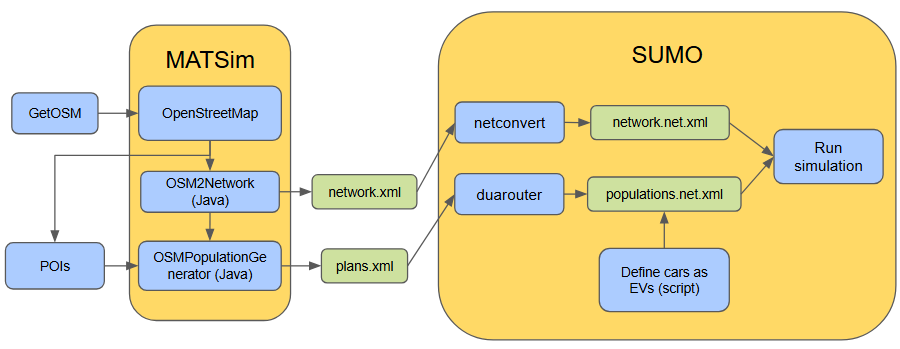
\includegraphics[width=\textwidth]{images/Bild_MATSim_SUMO_cut.png}
    \caption{Integration of MATSim \& SUMO}
    \label{fig:integration_matsim_sumo}
\end{figure}

The process begins with acquiring raw OSM data via the \texttt{GetOSM} script provided by SUMO. Then, the OpenStreetMap data is entered into MATSim, where it is parsed to construct a MATSim-like network model. Next, the \texttt{OSM2Network} Java module converts the model into a SUMO-compatible \texttt{network.xml} file.\newline
Meanwhile, the \texttt{OSMPopulationGenerator} creates an initial set of activity plans, which are serialized as \texttt{plans.xml}.

Once both files are produced, the workflow transitions to SUMO. The \texttt{netconvert} tool ingests the \texttt{network.xml} file from MATSim and outputs a SUMO-native \texttt{network.net.xml} file. Meanwhile, the \texttt{duarouter} tool takes the \texttt{plans.xml} file and generates the corresponding vehicle routes in the \texttt{populations.net.xml} file. A short post-processing script marks all passenger vehicles in the SUMO network as electric vehicles (EVs). Finally, the enriched network and routed population files are loaded into SUMO’s simulation engine for execution.

Coupling MATSim’s demand generator with SUMO’s detailed simulation creates a modular, reproducible pipeline that handles both large-scale scenarios and individual vehicle behavior - ideal for EV studies. All intermediate files are archived, and MATSim strategies or SUMO driver models can be tuned independently. Key challenges might become the error-prone conversions of MATSim files into SUMO-compatible files.

\subsubsubsection{Combination of BEAM and SUMO}
In general, using BEAM and SUMO together would be very similar to using MATSim and SUMO. BEAM would also use the OSM file to create a MATSIM-like network and population. After conversion, the workflow would also label the vehicles as EVs and run the simulation.

However, the key difference is that SUMO acts as a low-level traffic engine with a feedback loop to BEAM. At each simulation step, BEAM pauses SUMO via TraCI. Then, it retrieves vehicle states (position, speed, battery state of charge (SoC), and charger queues). After that, it updates agent decisions (energy consumption, charger detours, dynamic re-routing, and mode changes). Finally, it pushes those control commands back into SUMO.

\begin{figure}[ht]
    \centering
    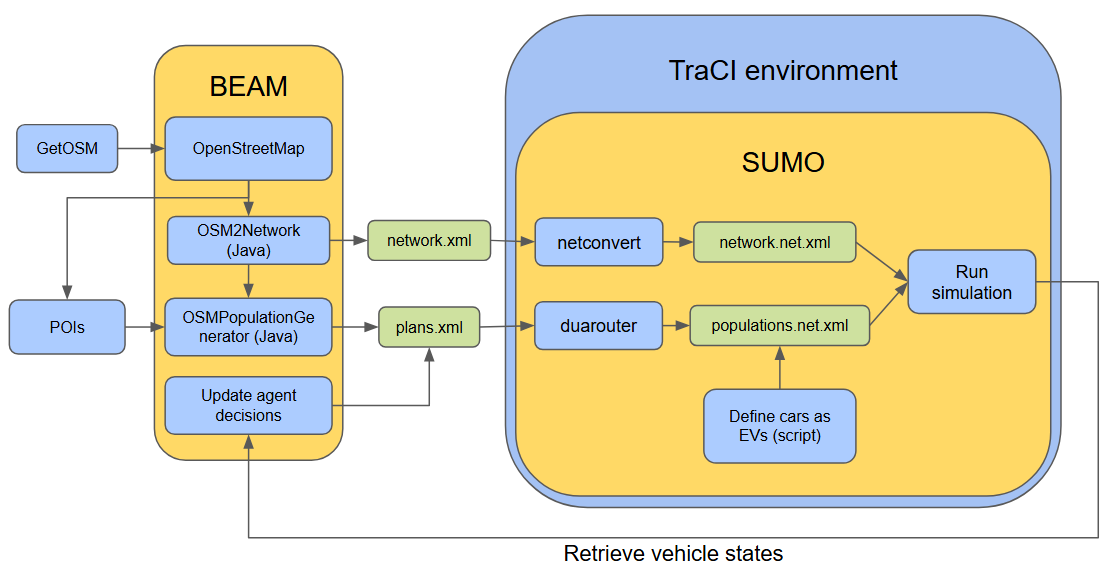
\includegraphics[width=\textwidth]{images/Bild_BEAM_SUMO.png}
    \caption{Integration of BEAM \& SUMO}
    \label{fig:integration_beam_sumo}
\end{figure}

This tight, real-time exchange ensures charging events, congestion avoidance, and routing adjustments happen in real time. Rather than relying on a single, static routing pass, the simulation constantly "comes back" to BEAM to refine every vehicle’s behavior.

Implementing a real-time feedback loop between MATSim and SUMO would add unnecessary overhead, since MATSim’s day-to-day replanning already produces optimized plans that SUMO simply executes. A continuous Java to TraCI bridge would introduce extra inter-process messaging and callback wiring without yielding new insights.

\subsubsection{Comparison of introduced concepts}
The following section compares the technologies presented and possible combinations and evaluates them based on various criteria. Some of these criteria are quantitative, while others are based on personal trial and error and experience.
   
% define a p‐column that is centered AND breaks lines automatically
\newcolumntype{C}[1]{>{\centering\arraybackslash}p{#1}}
\newcolumntype{G}{>{\columncolor{gray!20}\raggedright\arraybackslash}l}
\begin{landscape}
  \begin{table}[!htbp]
    \centering
    \small
    % tweak inter‐column gap if needed
    \setlength{\tabcolsep}{6pt}
    % we have 5 columns: 1 left‐aligned + 4 centered p‐columns of equal width
    % each C{<width>} will wrap text at word boundaries
    \begin{tabular}{|G|C{3.5cm}|C{3.5cm}|C{3.5cm}|C{3.5cm}|}
      \hline
      \rowcolor{gray!20}
      Criteria                   & \textbf{SUMO} 
                                 & \textbf{SAGA} 
                                 & \textbf{MATSim+SUMO} 
                                 & \textbf{BEAM+SUMO}     \\ \hline
      \textbf{OSM Import}        & \checkmark    
                                 & \checkmark    
                                 & \checkmark           
                                 & \checkmark             \\ \hline
      \textbf{Network Conversion}& \checkmark\ via netconvert   
                                 & \checkmark\ full OSM to SUMO pipeline   
                                 & (\checkmark) via OSM2Network (Java converter) 
                                 & (\checkmark) via OSM2Network (Java converter)  \\ \hline
      \textbf{Demand Generation} & (\checkmark) randomTrips only, or custom scripts    
                                 & \checkmark\ activity chains    
                                 & \checkmark\ co-evolutionary plans    
                                 & \checkmark\ activity \& RL-learned  \\ \hline
      \textbf{Temporal Realism}  & X (no built‐in schedules, only with custom scripts) 
                                 & \checkmark\ rush-hour noise + dwell 
                                 & \checkmark\ dynamic daily replanning 
                                 & \checkmark\ on-the-fly replanning     \\ \hline
      \textbf{Multimodal Support}& \checkmark\ cars, PT, bikes, pedestrians  
                                 & \checkmark\ multi-modal by default 
                                 & \checkmark\ multiple modes 
                                 & (\checkmark) mostly vehicles \\ \hline
      \textbf{Real-Time API}     & \checkmark\ TraCI 
                                 & \checkmark\ TraCI 
                                 & (\checkmark) only in the SUMO stage (TraCI)
                                 & \checkmark\ tight feedback loop via TraCI + BEAM \\ \hline
      \textbf{Extensibility \& Scripting}
                                 & CLI, Python scripts 
                                 & CLI + JSON configs + Python 
                                 & Java APIs, Python scripts 
                                 & Java + Python bindings \\ \hline
      \textbf{Documentation}
                                 & Excellent docs
                                 & Not well-documented
                                 & Mature docs
                                 & Active docs \\ \hline
      \textbf{Flexibility}       & \checkmark    & \checkmark    & \checkmark    & \checkmark              \\ \hline
      \textbf{App Possibilities} & general traffic sim
                                 & activity-based scenarios
                                 & research, large-scale planning
                                 & EV \& energy system studies   \\ \hline
      \textbf{Realism}           & basic realism
                                 & high realism
                                 & very high realism
                                 & very high realism             \\ \hline
      \textbf{Performance}       & fast C\texttt{++} core
                                 & Python/Java overhead
                                 & JVM + SUMO overhead
                                 & -   \\ \hline
      \textbf{Complexity}        & moderate
                                 & higher setup complexity
                                 & quite complex
                                 & very high complexity    \\ \hline
      \textbf{Notable Extras}    & osmWebWizard, osmGet/osmBuild 
                                 & Auto-POI extraction; TAZ weighting 
                                 & Large-scale OD matrices; plan-iteration 
                                 & EV charging RL; dynamic rerouting \\ \hline
    \end{tabular}
    \caption{Comparison of SUMO, SAGA, MATSim + SUMO, BEAM + SUMO}
  \end{table}
\end{landscape}

SUMO is undoubtedly the most efficient and flexible option as a standalone simulation tool. The C++-based engine allows for high performance, and CLI commands and provided or custom Python scripts allow for large-scale network or behavior adaptations.

With the \texttt{osmWebWizard}, the entire workflow - from selecting and downloading the OSM map to setting attributes such as the simulation duration and finally starting the SUMO GUI - becomes easy.

However, there are no native mechanisms for generating demand beyond random trips and fixed daily or weekly cycles. Functions such as electric vehicles and on-the-fly replanning must be developed and integrated. While it offers more flexibility, it significantly increases the implementation effort and long-term maintenance requirements.

SAGA extends SUMO by providing a fully integrated OSM-to-SUMO pipeline that automatically extracts points of interest (POIs), allocates and weights traffic analysis zones (TAZ), and generates activity chains. Through this end-to-end preprocessing, it produces travel demand profiles with realistic daily patterns.

While the additional preprocessing stage introduces only a moderate performance overhead, SAGA remains fully open-source and can be customized via SUMO’s TraCI interface to accommodate project-specific requirements. However, the existing user documentation contains significant gaps that hinder rapid onboarding, and built-in error-handling routines are currently insufficient for robust, large-scale applications.

MATSim and SUMO integrate the strengths of large-scale, agent-based demand modeling with a high-performance microscopic execution engine. Networks of large size can be imported directly from OpenStreetMap into MATSim, where optimized agents’ daily plans are generated based on activity schedules. These precomputed plans are then executed in SUMO, leveraging its performant core for vehicle kinematics.

During runtime, the TraCI interface enables dynamic interventions — vehicles can be rerouted in response to emerging congestion, and battery state-of-charge (SoC) can be monitored and controlled for electric-vehicle fleets. 
Nevertheless, it should be noted that most of the routing logic is done in MATSim and SUMO itself only acts as a fast execution layer. This separation can limit the granularity of on-the-fly adaptations and may introduce additional complexity.

In addition to traffic simulation, BEAM integrates energy systems and offers electric vehicles (EVs) and charging infrastructure. However, the real-time loop between SUMO and BEAM, as well as the stepwise simulation, introduces massive overhead. This, coupled with the complex implementation, may make this combination a less attractive option for many projects.

\clearpage
\subsection{Charging Station Placement Algorithm}

\subsubsection{Requirements for Charging Station Placement Algorithm}

The placement algorithm must first perform clustering to detect EV-demand hotspots and then automatically propose new charging-point candidates. It should support exporting its findings in GeoJSON and XML, and use a multi-criteria optimization engine — balancing traffic flow, site accessibility and grid capacity to select locations. The system must be able to optimize toward different objectives, such as maximizing coverage or minimizing average user distance, and rank all proposed sites with a scoring metric. Finally, it should maintain detailed logs of every optimization run for auditing and analysis. 

Another aspect for placement is the consideration of a self-owned in-house wallbox or charging options at the work location, which a person might be more likely to use \cite{ev_cs_planning_with_dyn_pred}. This can be explained by the trip chain, which is consistent with people's daily travel law. Eventually, the placement and removing should be executed automatically, based on traffic, traffic flow, based on a realistic simulation \cite{cs_ev_in_SUMO_impact_on_traffic_flow}.

\subsubsection{Assumptions}

\subsubsubsection{Parking areas}
There are two main reasons why implementing realistic “parking-bay” chargers in SUMO is exceptionally difficult. First, SUMO’s network model is built around edges and lanes rather than individual parking stalls. In order to represent individual parking spots, each lot would need to be divided into dozens or hundreds of tiny edge segments and assigned its own links. Additionally, traffic lights or way logic would have to be implemented to prevent collisions, and a custom script would have to be created to handle the routing of EVs so they can actually park in those bays. This would greatly increase development time and the risk of errors.

Second, SUMO’s electric-vehicle extension only supports chargers attached to lanes or edges. There is no built-in mechanism for "off-lane" or stationary charging.

For these reasons, we assume that EVs charge in a special "charging lane" rather than in separate parking bays. Vehicles simply pull into that lane; SUMO’s existing battery and charger modules work unmodified; and we avoid custom network-generation scripts while still capturing the key effects of charging stops on routing and traffic flow.

\subsubsubsection{Points of Interests}
Certain areas can be considered points of interest. Namely, work location, shopping locations, residential areas or home addresses, to be more specific and others, that qualify. It is reasonable to believe, that the extraction of points of interest from the OSM will offer a wide range of potential improvements to the system. For example when trying to optimize traffic and maybe even go so far, to say that cars can and should be assigned specific charging stations, that potentially are not the closest, but most optimal - considering waiting time, distance, travel time and other factors \cite{wevj14020040}. Currently points of interest have no inherent value or use, when looking at the documentation of SUMO itself, "definitions of colored polygons and POIs (points of interest) can be loaded within an additional-file. These shapes are currently meant to improve a simulation's appearance and to allow an easier debugging. No special interaction with them is implemented, yet" \cite{sumo_shapes}.

\subsubsection{Charging Station Algorithm}
The rationale behind the Charging Station Placement Algorithm is primarily to identify optimal locations for charging stations (CS) that reliably capture high traffic volumes and minimize waiting times. To emphasize the importance of traffic patterns, Figure \ref{fig:heatmapRoads} presents a heatmap of heavily used roads, while Figure \ref{fig:heatmapResidents} shows the residential origins of travelers, which helps explain certain red edges in the road heatmap. Naturally, placing CS near roads with high vehicle throughput is a sensible approach, as most drivers are likely to pass through these areas. However, exploring ways to better distribute that traffic may be even more effective in reducing waiting times.

\begin{figure}[ht]
    \centering
    \begin{subfigure}[b]{0.36\textwidth}
        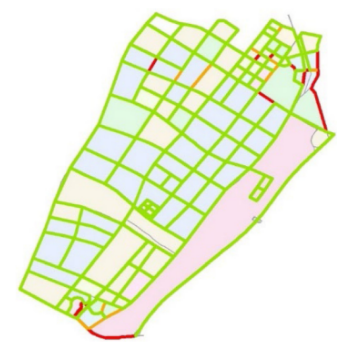
\includegraphics[width=\textwidth]{images/heatmapRoads.png}
        \caption{Heatmap of Road Usage}
        \label{fig:heatmapRoads}
    \end{subfigure}
    \hspace{5pt}  % kleiner Abstand
    \begin{subfigure}[b]{0.36\textwidth}
        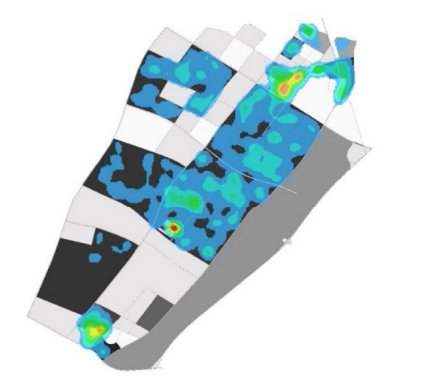
\includegraphics[width=\textwidth]{images/heatmapResidents.png}
        \caption{Heatmap of Residency}
        \label{fig:heatmapResidents}
    \end{subfigure}
    \caption{Comparison of Heatmaps for Roads and Residency}
    \label{fig:heatmapsComparison}
\end{figure}

Due to the objective, an iterative approach seems well-fit to satisfy the requirements. The CS will be randomly placed, as it cannot be anticipated how the lanes are built, before the first iteration of the simulation and after it has finished, the data will be logged to extract information from, which will be used to improve the existing system.
Certain locations, such as remote areas along highways, may not be considered for charging station placement if they are unlikely to reach the required usage levels. To combat that potential error, implementing machine learning could be a big step, to account for uncertainty, improve positioning of CS with actual traffic flow, density and occupancy of roads themselves \cite{vazifeh2015optimizing}.

\subsection{Integration of Grid Models}
\subsubsection{Requirements for Integration of Grid Models}
For the efficient operation of vehicle-to-grid (V2G) systems, it is essential to integrate grid-relevant data into the optimization process for the charging infrastructure. As already described in the requirements above, the locations of charging stations should also be optimized in relation to existing grid capacity. Grid conditions should be taken into account in order to reduce grid loads and avoid charging peaks. This is to ensure that charging points are not only user-friendly but also positioned in a way that is compatible with the grid.

\subsubsection{Approaches to integrate V2G functionality}
SUMO itself does not natively support direct integration for connecting or simulating electrical networks. Therefore, a third-party or proprietary implementation is necessary. The following describes possible approaches that could implement V2G functionality, but these will be further validated in upcoming research phases.

\subsubsubsection{Integration of Power Lines into Simulation Network}
Although SUMO does not offer native support for power grids, power lines can still be modeled. This can be done, for example, using the \texttt{netedit} tool provided by SUMO. The power lines are integrated into the existing road network as special edges with the attribute \texttt{type="powerline"}. In this way, both fictitious and real power grids can be integrated into the simulation and visualized.

To evaluate the location of a planned charging station, Python scripts can be used to check whether the station is sufficiently close to a power line using geometric calculations. If the distance is below a defined threshold (e.g., 50 meters), the location can be considered suitable - otherwise, it is rejected.

This method serves as an efficient pre-filter when planning charging infrastructure, especially for large-scale networks or urban scenarios.

\subsubsubsection{Runtime Monitoring of Grid Loads}
SUMO maps the charging process of electric vehicles, but does not simulate physical loads or capacities of the power grid. In order to evaluate a charging station during runtime based on grid capacity, SUMO could be extended with internal control logic via a TraCI interface.

This would involve implementing a state memory for each charging station during runtime, which would record how many EVs are charging at any given time, how much electrical power is being drawn, and whether the station is considered overloaded. In vehicle-to-grid scenarios, it would also be possible to document whether vehicles are feeding energy back into the grid.

This data enables a detailed analysis of the temporal load distribution at individual stations. This allows overload situations to be detected, not often used stations to be identified, and possible measures for optimizing performance, number, or location to be derived.

An extended version of this approach involves linking to an external grid model, e.g., via \texttt{pandapower}. The charging stations are mapped as nodes (buses) in the electrical grid. A network calculation is performed for each new charging request \cite{noauthor_pandapower_nodate, noauthor_about_nodate}. If the additional consumption leads to overvoltage or overload, the charging process can be specifically prevented in SUMO or rejected by the station.

This approach would make it possible to take into account not only the location of charging stations, but also the technical limitations of the power grid.

